\section{Introduzione}
\begin{frame}{}

  \textsc{Green Together} permette di semplificare la trasmissione dell'informazione da e verso i cittadini, includendoli e ascoltandoli.
  \pause
  \bigskip

  Un canale a doppio flusso che semplifica e centralizza la comunicazione.

\end{frame}
\begin{frame}
  Non sarà più necessario analizzare grosse quantità di mail per capire quali siano le richieste ricorrenti e cosa stia davvero a cuore ai cittadini
  \pause

  Con un'unica piattaforma sarà possibile esercitare:
  \begin{itemize}
    \item informazione
    \item trasparenza
    \item privacy
    \item partecipazione
  \end{itemize}

\end{frame}
\begin{frame}{Attori}
  Gli attori che entrano in gioco sono:
  \begin{description}
    \item[I cittadini] che usufruiscono dei servizi ambientali di zona
    \item[L'azienda] che gestisce questi servizi
  \end{description}


\end{frame}

\begin{frame}{Struttura}

  \begin{figure}

    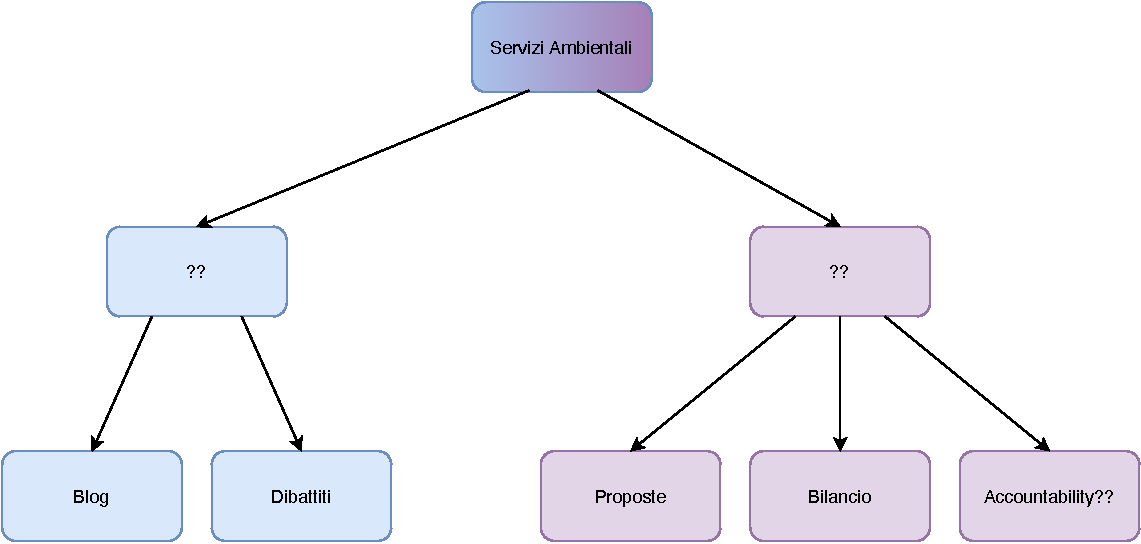
\includegraphics[width=\textwidth]{Diagramma}
  \end{figure}

\end{frame}
\begin{frame}{Funzioni}
  \alert{Dialoghiamo}

  \begin{description}
    \item[Blog] Consente all'\textbf{azienda} di comunicare con i \textbf{cittadini}
    \item[Dibattiti] Consente ai \textbf{cittadini} di comunicare reciprocamente e con l'\textbf{azienda}
  \end{description}

  \alert{Decidiamo}

  \begin{description}
    \item[Proposte] Consente ai cittadini e all'azienda di fare proposte e votarle
    \item[Bilancio] Una volta selezionate alcune proposte consente di ripartire un budget sui vari progetti
    \item[Accountability] Monitora lo stato dei progetti sovvenzionati
  \end{description}

\end{frame}